\documentclass{article}

% Language setting
% Replace `english' with e.g. `spanish' to change the document language
\usepackage[english]{babel}
\usepackage{float}

% Set page size and margins
% Replace `letterpaper' with `a4paper' for UK/EU standard size
\usepackage[letterpaper,top=2cm,bottom=2cm,left=3cm,right=3cm,marginparwidth=1.75cm]{geometry}

% Useful packages
\usepackage{amsmath}
\usepackage{graphicx}
\usepackage[colorlinks=true, allcolors=blue]{hyperref}
\usepackage{titling}

\setcounter{section}{-1}

\title{
\includegraphics[scale=0.5]{logo.jpg}\\ \textbf{Laboratorio 1} 
\\ \large Introducción - Errores - Álgebra Lineal                   
\\ \large Métodos de Computación Científica}

\author{Manuel Lagos}

\begin{document}
\maketitle

\section{Introduction}

Los ejercicios del laboratorio fueron resueltos utilizando el software sugerido Octave y fueron incluidas capturas de pantallas del código escrito y el resultado obtenido con el programa. El trabajo fue realizado con un $\epsilon_{mach}$ de $2^{-5}$ en una computadora de 64 bits.

\section{Ejercicio 1}
Se evaluó la función $f(x)=x^3-3x^2+3x-1$ en el intervalo $[0, 2]$ con un paso $h=0.001$, y se obtuvo un resultado esperable. Luego, fue evaluada alrededor de $x=1\pm0.000025$ en 640 puntos distintos, logrando el efecto de nube de puntos con el objetivo de reproducir el fenómeno visto en la teoría como \textit{“Ruido en la evaluación de funciones}”. La banda difusa de puntos de este segundo resultado presenta una dificultad para determinar la raíz del polinomio en cuestión, no está claro dónde interseca el eje de las abscisas. 

De manera similar se procedió con la función $f(x)=x^3+2x^2-x-2$, sin embargo se obtuvieron distintos resultados. En este segundo experimento, la banda de puntos sí logra evidenciar la raíz del polinomio, aún con una cantidad escasa de puntos.

La diferencia entre ambos resultados se puede explicar por la inclinación que presentan los polinomios alrededor de la raíz. En el primer caso, al haber un punto de inflexión sobre la raíz, la función es prácticamente indistinguible del eje en un entorno del punto, y es esta falta de diferencia lo que dificulta determinar el punto de intersección. En cambio, en el segundo caso la función pasa por el eje con una inclinación bien marcada y la raíz puede ser determinada sin dificultad. 

\begin{figure}[H]
    \centering
    \includegraphics[width=1\linewidth]{ej1.gráfico1.1.png}
    \caption{$f(x)=x^3-3x^2+3x-1$ en $[0, 2]$ con un paso $h=0.001$}
    \label{fig:enter-label}
\end{figure}

\begin{figure}[H]
    \centering
    \includegraphics[width=1\linewidth]{ej1.código1.1.png}
    \caption{Código de la figura anterior}
    \label{fig:enter-label}
\end{figure}

\begin{figure}[H]
    \centering
    \includegraphics[width=1\linewidth]{ej1.gráfico1.2.png}
    \caption{$f(x)=x^3-3x^2+3x-1$ evaluada alrededor de $x=1\pm0.000025$ en 640 puntos}
    \label{fig:enter-label}
\end{figure}

\begin{figure}[H]
    \centering
    \includegraphics[width=1\linewidth]{ej1.código1.2.png}
    \caption{Código de la figura anterior}
    \label{fig:enter-label}
\end{figure}

\begin{figure}[H]
    \centering
    \includegraphics[width=1\linewidth]{ej1.gráfico2.1.png}
    \caption{$f(x)=x^3+2x^2-x-2$ en $[0, 2]$ con un paso $h=0.001$}
    \label{fig:enter-label}
\end{figure}

\begin{figure}[H]
    \centering
    \includegraphics[width=1\linewidth]{ej1.código2.1.png}
    \caption{Código de la figura anterior}
    \label{fig:enter-label}
\end{figure}

\begin{figure}[H]
    \centering
    \includegraphics[width=1\linewidth]{ej1.gráfico2.2.png}
    \caption{$f(x)=x^3+2x^2-x-2$ evaluada alrededor de $x=1\pm0.000025$ en 300 puntos}
    \label{fig:enter-label}
\end{figure}

\begin{figure}[H]
    \centering
    \includegraphics[width=1\linewidth]{ej1.código2.2.png}
    \caption{Código de la figura anterior}
    \label{fig:enter-label}
\end{figure}

\section{Ejercicio 2}
Se realizó un programa para construir la matriz de Hilbert con n=20, y se calcularon sus autovectores y sus autovalores asociados empleando las funciones provistas por el software.\\

\begin{equation}
    \centering
    H_{ij} = \dfrac{1}{i+h-1}
\end{equation}\\

La matriz de Hilbert es un conocido ejemplo de una matriz mal condicionada, lo que significa que es especialmente sensible a pequeñas perturbaciones numéricas en la entrada. Esto la hace una matriz problemática para trabajar en aplicaciones numéricas. \\

\textit{aclaración: Los autovectores se observan como los vectores columna que conforman la matriz autovectores. El n-ésimo autovector está asociado al elemento de la matriz columna de autovalores de la n-ésima fila.}
	
\begin{figure}[H]
    \centering
    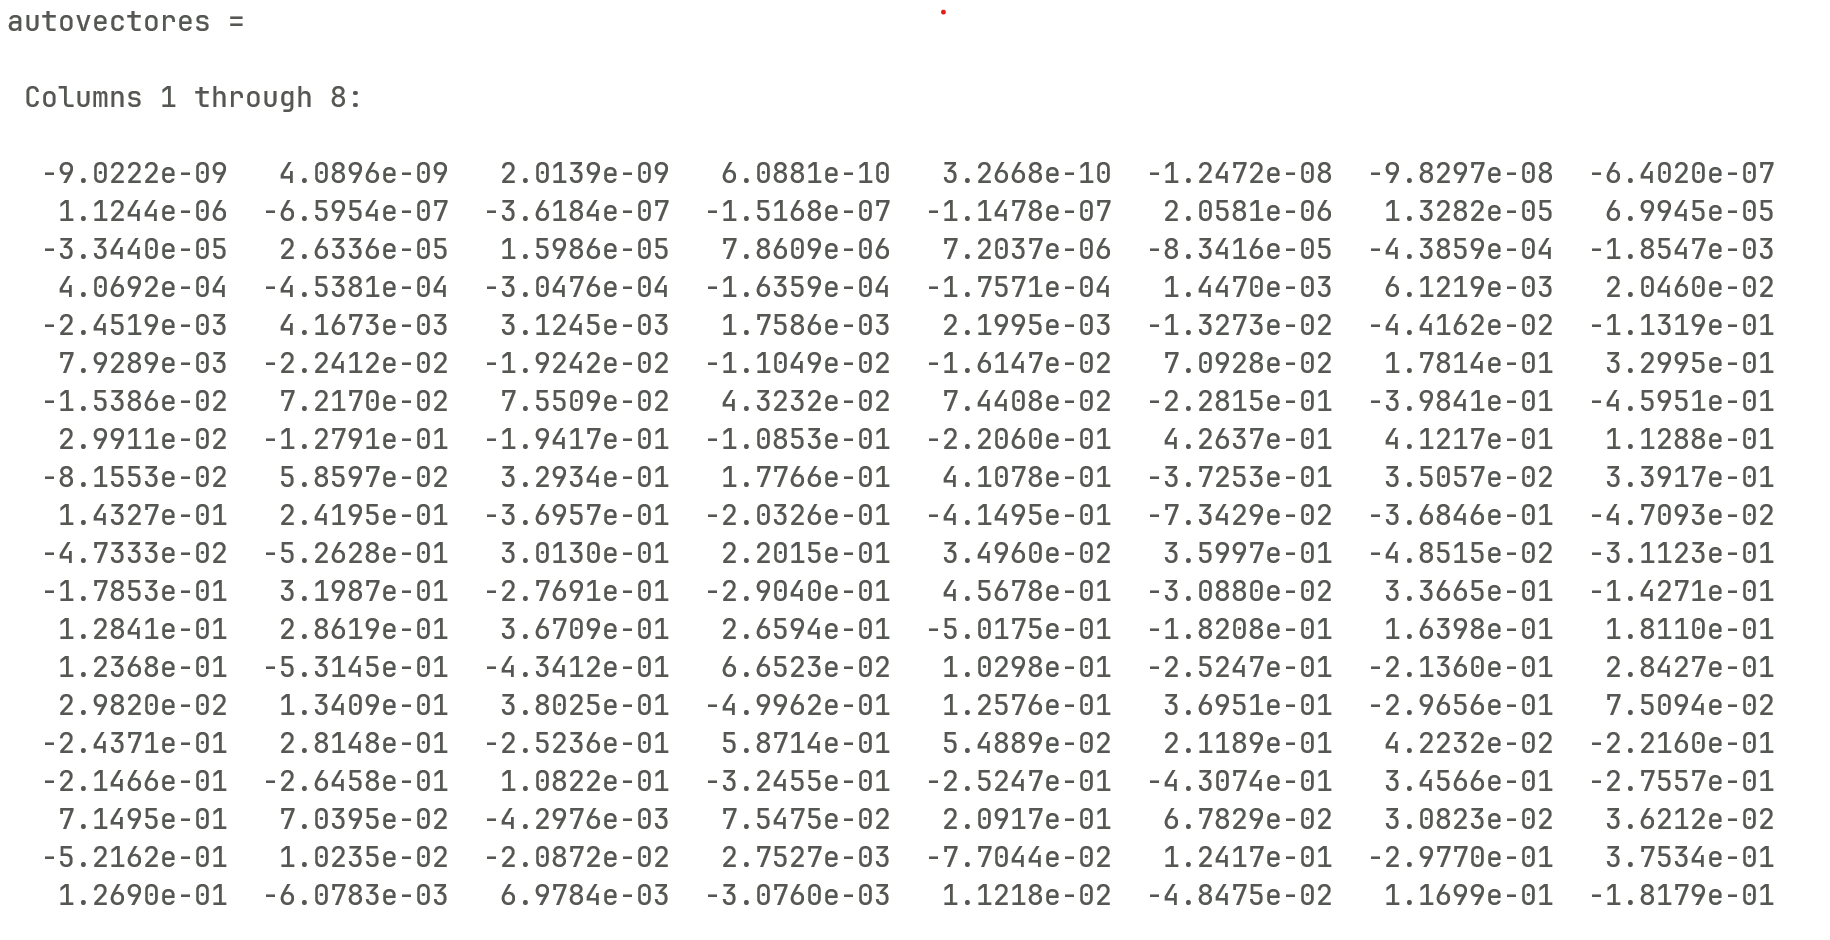
\includegraphics[width=1\linewidth]{ej2.resultado.1.png}
    \caption{Autovectores de $H_{20}$ de 1 a 8}
    \label{fig:enter-label}
\end{figure}

\begin{figure}[H]
    \centering
    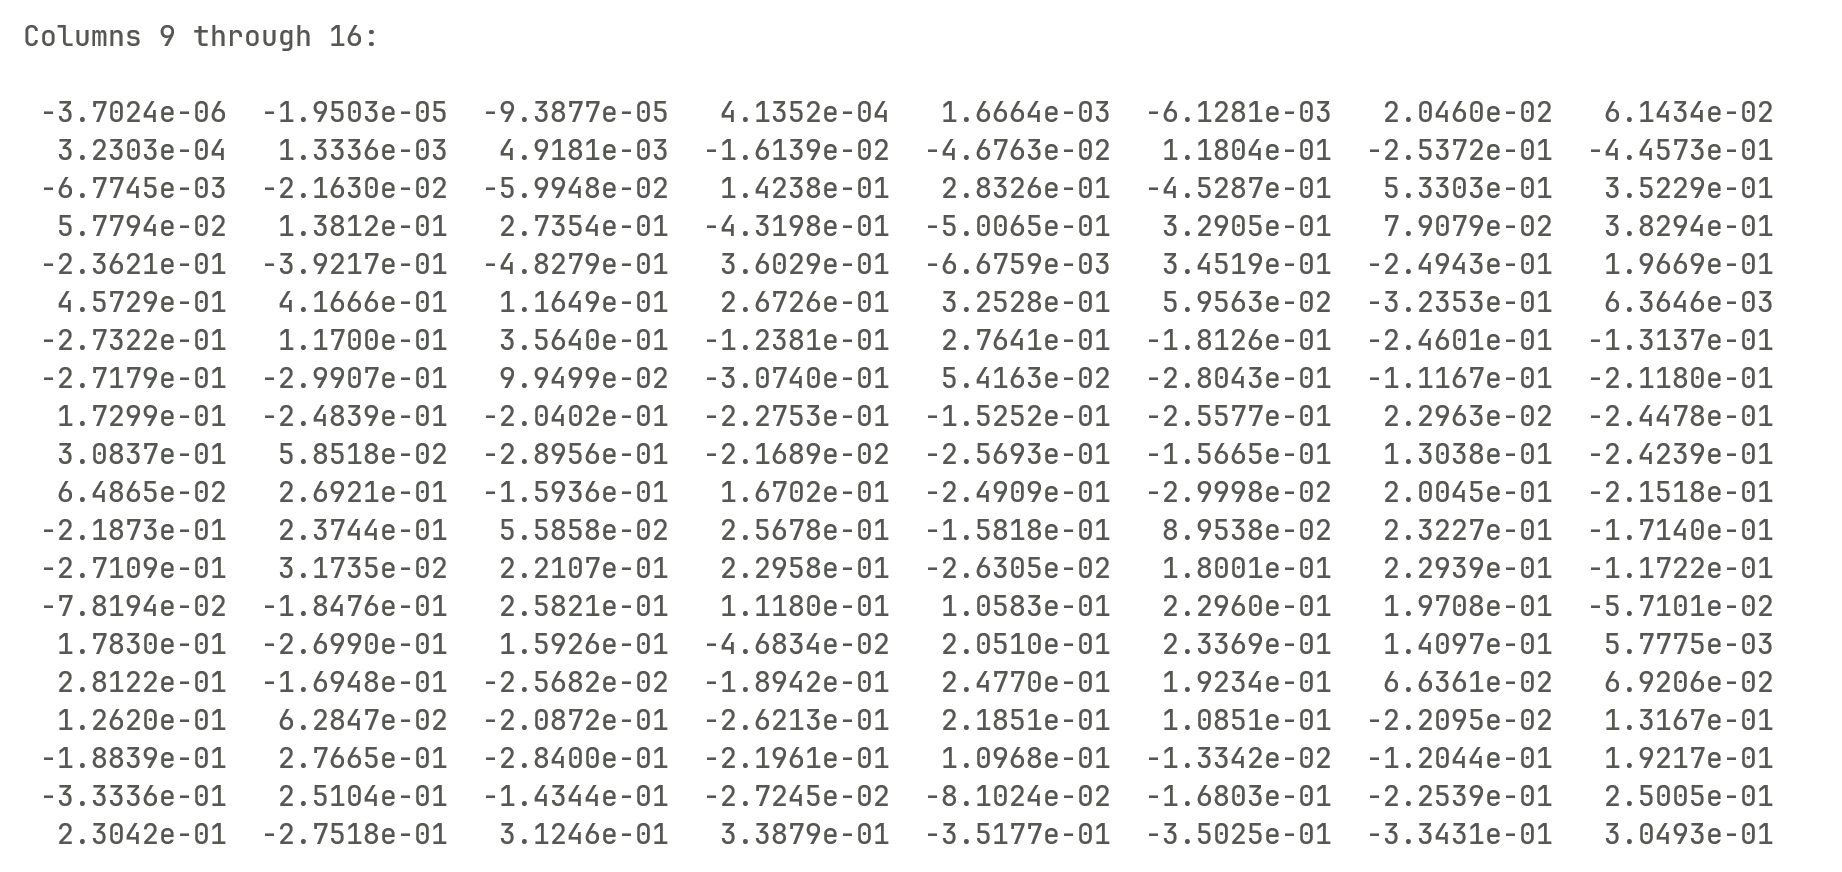
\includegraphics[width=1\linewidth]{ej2.resultado.2.png}
    \caption{Autovectores de $H_{20}$ de 9 a 16}
    \label{fig:enter-label}
\end{figure}

\begin{figure}[H]
    \centering
    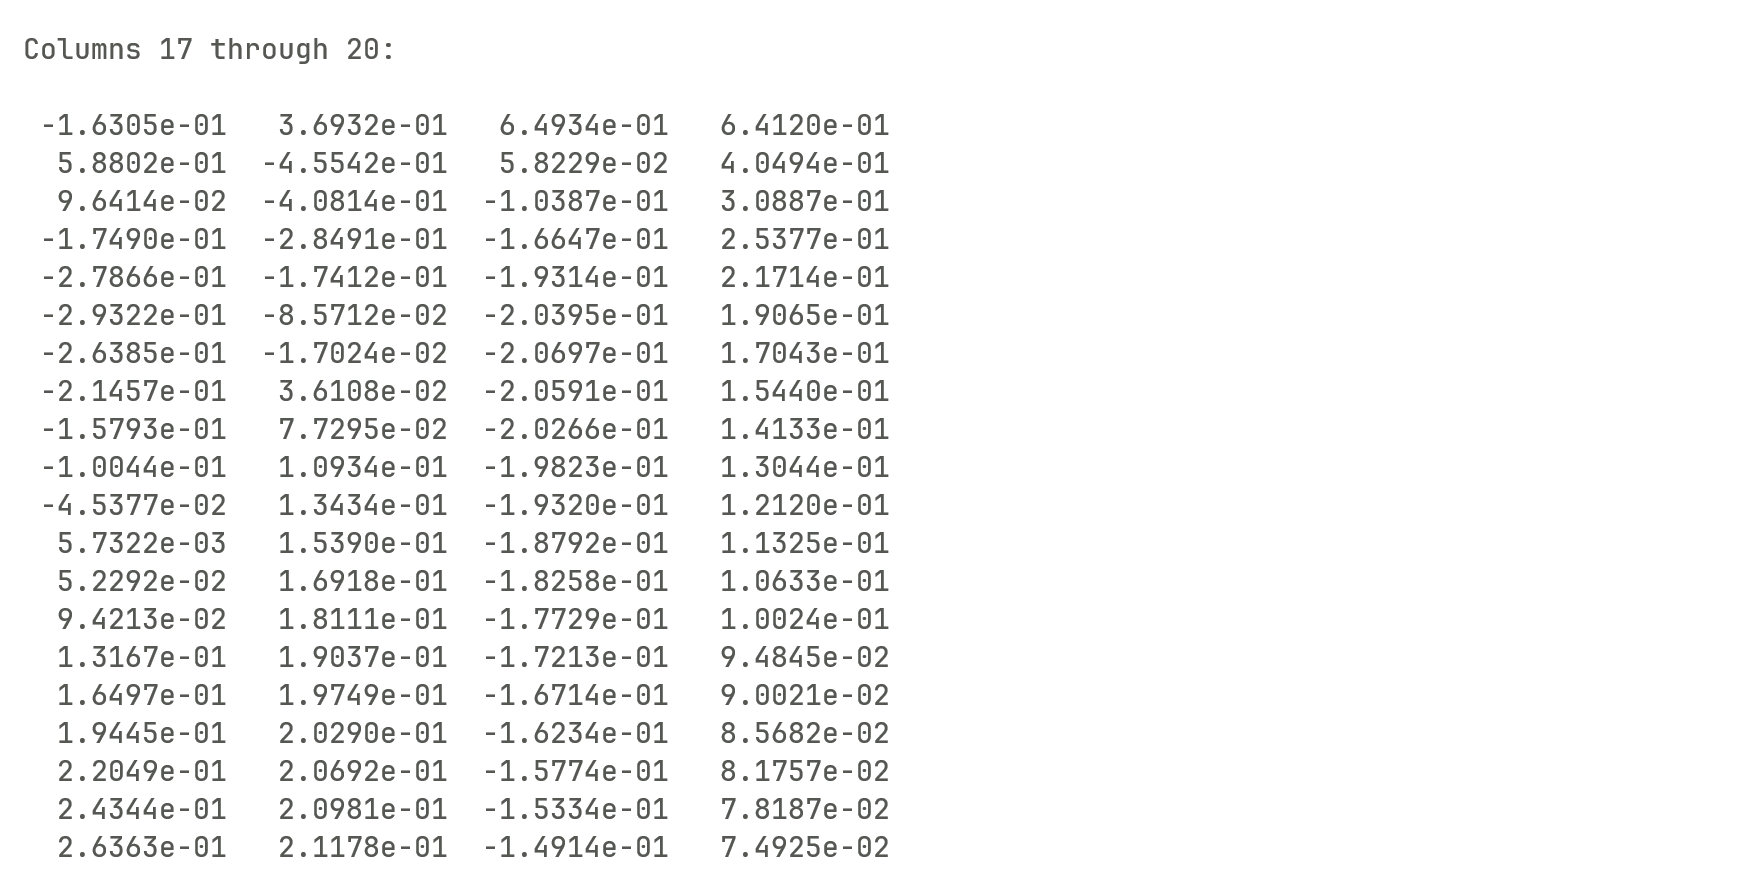
\includegraphics[width=1\linewidth]{ej2.resultado.3.png}
    \caption{Autovectores de $H_{20}$ de 17 a 20}
    \label{fig:enter-label}
\end{figure}

\begin{figure}[H]
    \centering
    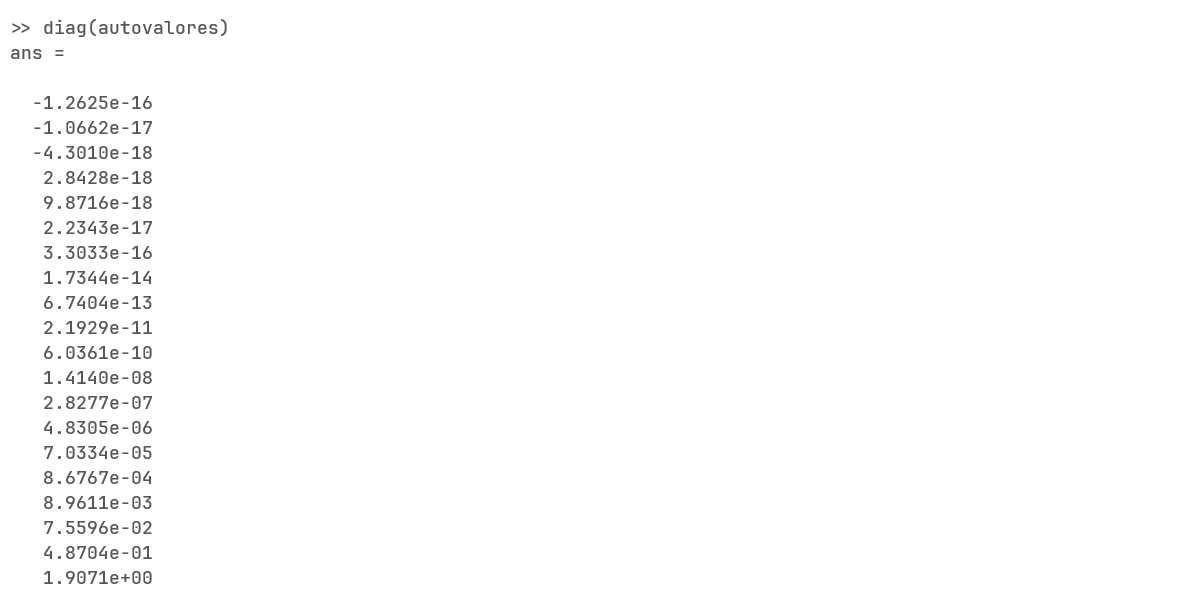
\includegraphics[width=1\linewidth]{ej2.resultado.4.png}
    \caption{Autovalores de $H_{20}$.}
    \label{fig:enter-label}
\end{figure}

\begin{figure}[H]
    \centering
    \includegraphics[width=1\linewidth]{ej2.código.png}
    \caption{Código del programa}
    \label{fig:enter-label}
\end{figure}

\section{Ejercicio 3}
Se escribió un programa para aproximar la derivada de la función $f(x)=tan(x)$ en $x=1$ empleando primero la fórmula de diferencias finitas hacia adelante, y luego la fórmula de diferencias finitas centrales, en ambas ocasiones computando 100 puntos. También, se graficó para cada una la magnitud del error absoluto con respecto al valor real de la derivada en función del paso h utilizado, en una escala logarítmica de ambos ejes para una correcta apreciación. Además, se calculó la mejor aproximación obtenida, su correspondiente error, y el paso h utilizado, y se lo comparó con el sugerido por la regla del pulgar $h\approx \sqrt{\epsilon_{mach}}$.\\

Los resultados del experimento muestran que la regla del pulgar obtiene mejores resultados con la fórmula de aproximación por diferencias finitas hacia adelante que con la de diferencias centrales, esto es así posiblemente porque fue hecha a medida para la primera fórmula y no así para la segunda.
	
\begin{figure}[H]
    \centering
    \includegraphics[width=1\linewidth]{ej3.gráfico.1.png}
    \caption{\textbf{Diferencias finitas hacia adelante}:  magnitud del error absoluto en función del paso h}
    \label{fig:enter-label}
\end{figure}

\begin{figure}[H]
    \centering
    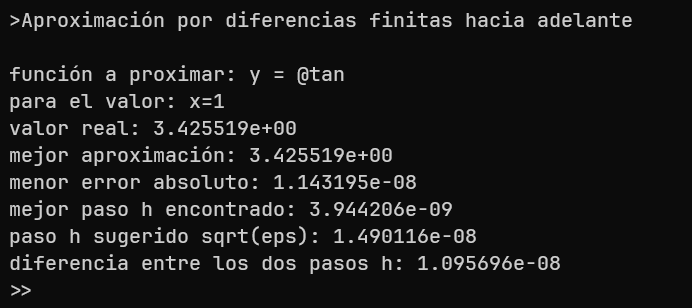
\includegraphics[width=1\linewidth]{ej3.resultados.1.png}
    \caption{Salida por consola}
    \label{fig:enter-label}
\end{figure}

\begin{figure}[H]
    \centering
    \includegraphics[width=1\linewidth]{ej3.código.1.png}
    \caption{Código de la figura anterior}
    \label{fig:enter-label}
\end{figure}

\begin{figure}[H]
    \centering
    \includegraphics[width=1\linewidth]{ej3.gráfico.2.png}
    \caption{\textbf{Diferencias finitas centrales}:  magnitud del error absoluto en función del paso h}
    \label{fig:enter-label}
\end{figure}

\begin{figure}[H]
    \centering
    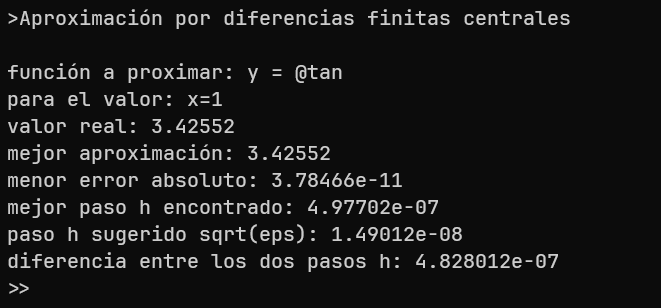
\includegraphics[width=1\linewidth]{ej3.resultados.2.png}
    \caption{Salida por consola}
    \label{fig:enter-label}
\end{figure}

\begin{figure}[H]
    \centering
    \includegraphics[width=1\linewidth]{ej3.código.2.png}
    \caption{Código de la figura anterior}
    \label{fig:enter-label}
\end{figure}

\section{Ejercicio 4}
Se realizó un programa para computar la serie infinita conocida como serie armónica $\sum_{n=1}^{\infty}1/n$, en simple y en doble precisión. La serie en cuestión es divergente. Sin embargo, puesto que se realizó la sumatoria con una precisión finita, se obtuvo un resultado finito. Podría pensarse que eventualmente el número $1/n$ será tan pequeño que producirá un undeflow, o que el contador $n$ será tan grande que producirá un overflow, estos superan las posibilidades de representación propias de la máquina. Aunque, de hecho, la sumatoria terminará antes de producirse cualquiera de estas dos excepciones, precisamente cuando 1/n resulte despreciable con respecto a la suma parcial. Esto es así debido a la operación de suma en punto flotante que debe igualar los exponentes perdiendo bits de la mantisa, y, eventualmente cuando la diferencia de magintud es muy grande, igualar el número más pequeño a cero. Esto ocurrirá puntualmente cuando $1/n < \epsilon_{mach}\sum_{k=1}^{n-1}(1/k)$. Luego la serie divergente resulta en una suma finita. Se realizó un gráfico de cómo crece la suma parcial en función de la n-ésima iteración para una mejor apreciación.

Para la sumatoria en doble precisión se procedió de manera similar pero estableciendo un criterio de parada al tratarse de un problema de mayor complejidad computacional, al menos para las computadoras actuales. El experimento fue interrumpido abrutamente a las siete horas de haber comenzado por cuestiones de limitaciones técnincas, el mismo no solo insumió mucho tiempo sino que también ocupó gran cantidad de la memoria de la máquina, y fue trabajoso luego reconstrir los datos obtenidos para generar el gráfico. 

Como conclusión, con la aritmética de doble precisión se obtiene una considerable mejora en la precisión de los cálculos pero implica un mayor consumo de los recursos de la máquina, afectando por tanto al tiempo de cómputo. Este \textit{tradeoff} debe ser tenido en cuenta en cada caso particular de aplicación.

\begin{figure}[H]
    \centering
    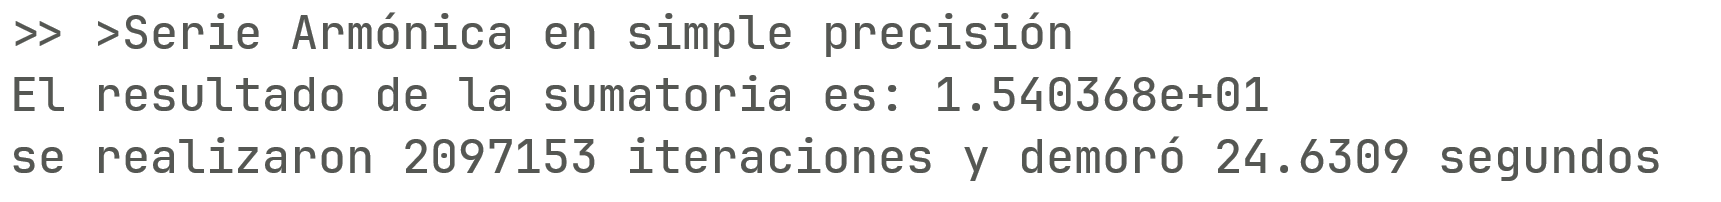
\includegraphics[width=1\linewidth]{ej4.resultado.1.png}
    \caption{Sumatoria Serie Armónica $\sum_{n=1}^{\infty}1/n$ en precisión simple.}
    \label{fig:enter-label}
\end{figure}

\begin{figure}[H]
    \centering
    \includegraphics[width=1\linewidth]{ej4.gráfico.1.png}
    \caption{Suma parcial en función de la n-ésima iteración}
    \label{fig:enter-label}
\end{figure}

\begin{figure}[H]
    \centering
    \includegraphics[width=1\linewidth]{ej4.código.1.png}
    \caption{Código de la figura anterior}
    \label{fig:enter-label}
\end{figure}

\begin{figure}[H]
    \centering
    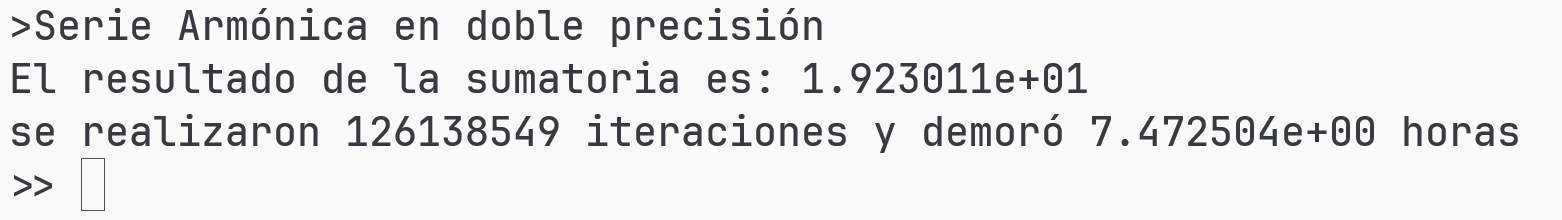
\includegraphics[width=1\linewidth]{ej4.resultado.2.png}
    \caption{Sumatoria Serie Armónica $\sum_{n=1}^{\infty}1/n$ en precisión doble acotada.}
    \label{fig:enter-label}
\end{figure}

\begin{figure}[H]
    \centering
    \includegraphics[width=1\linewidth]{ej4.gráfico.2.png}
    \caption{Suma parcial en función de la n-ésima iteración}
    \label{fig:enter-label}
\end{figure}

\begin{figure}[H]
    \centering
    \includegraphics[width=1\linewidth]{ej4.código.2.png}
    \caption{Código de la figura anterior}
    \label{fig:enter-label}
\end{figure}

\section{Ejercicio 5}
Se realizó un programa para construir la matriz A propuesta con $n=50$ y calcular su inversa. Además, se calculó el error sumando todos los elementos de la matriz $C=A \cdot A^{-1}$ y se lo comparó con $I_{n}$.\\

Si $A^_{-1}$ fue correctamente calculada, entonces $C=A \cdot A^{-1}=I$. Luego,
la suma de los elementos de C debe ser igual a la suma de los elementos de $I_{50}$, esto es $\sum_{i=1}^{50}\sum_{j=1}^{50}Cij = 50$. Calculando C y la suma de sus elementos, y restándole 50 al resultado, se obtiene una medida del error.\\
\[
A=\begin{bmatrix}
$\dfrac{n+2}{2n+2}$ & -\dfrac{1}{2}$ & 0 & 0 & \dots & 0 & 0 & \dfrac{1}{2n+2}$ \\
-\dfrac{1}{2}$ & 1 & -\dfrac{1}{2}$ & 0 & \dots & 0 & 0 & 0 \\
0 & -\dfrac{1}{2}$ & 1 & -\dfrac{1}{2}$ & \dots & 0 & 0 & 0 \\
. & . & .& .& \dots & .& .& .& \\
.& .& .& .& \dots & .& .& .& \\
.& .& .& .& \dots & .& .& .& \\
.& .& .& .& \dots & .& .& .& \\
 0  & 0 & 0 & 0 & \dots & -\dfrac{1}{2}$ & 1 & -\dfrac{1}{2}$ \\
$\dfrac{1}{2n+2}$ & 0 & 0 & 0 & \dots & 0 & -\dfrac{1}{2}$ & \dfrac{n+2}{2n+2}$ \\
\end{bmatrix}
\]

\begin{figure}[H]
    \centering
    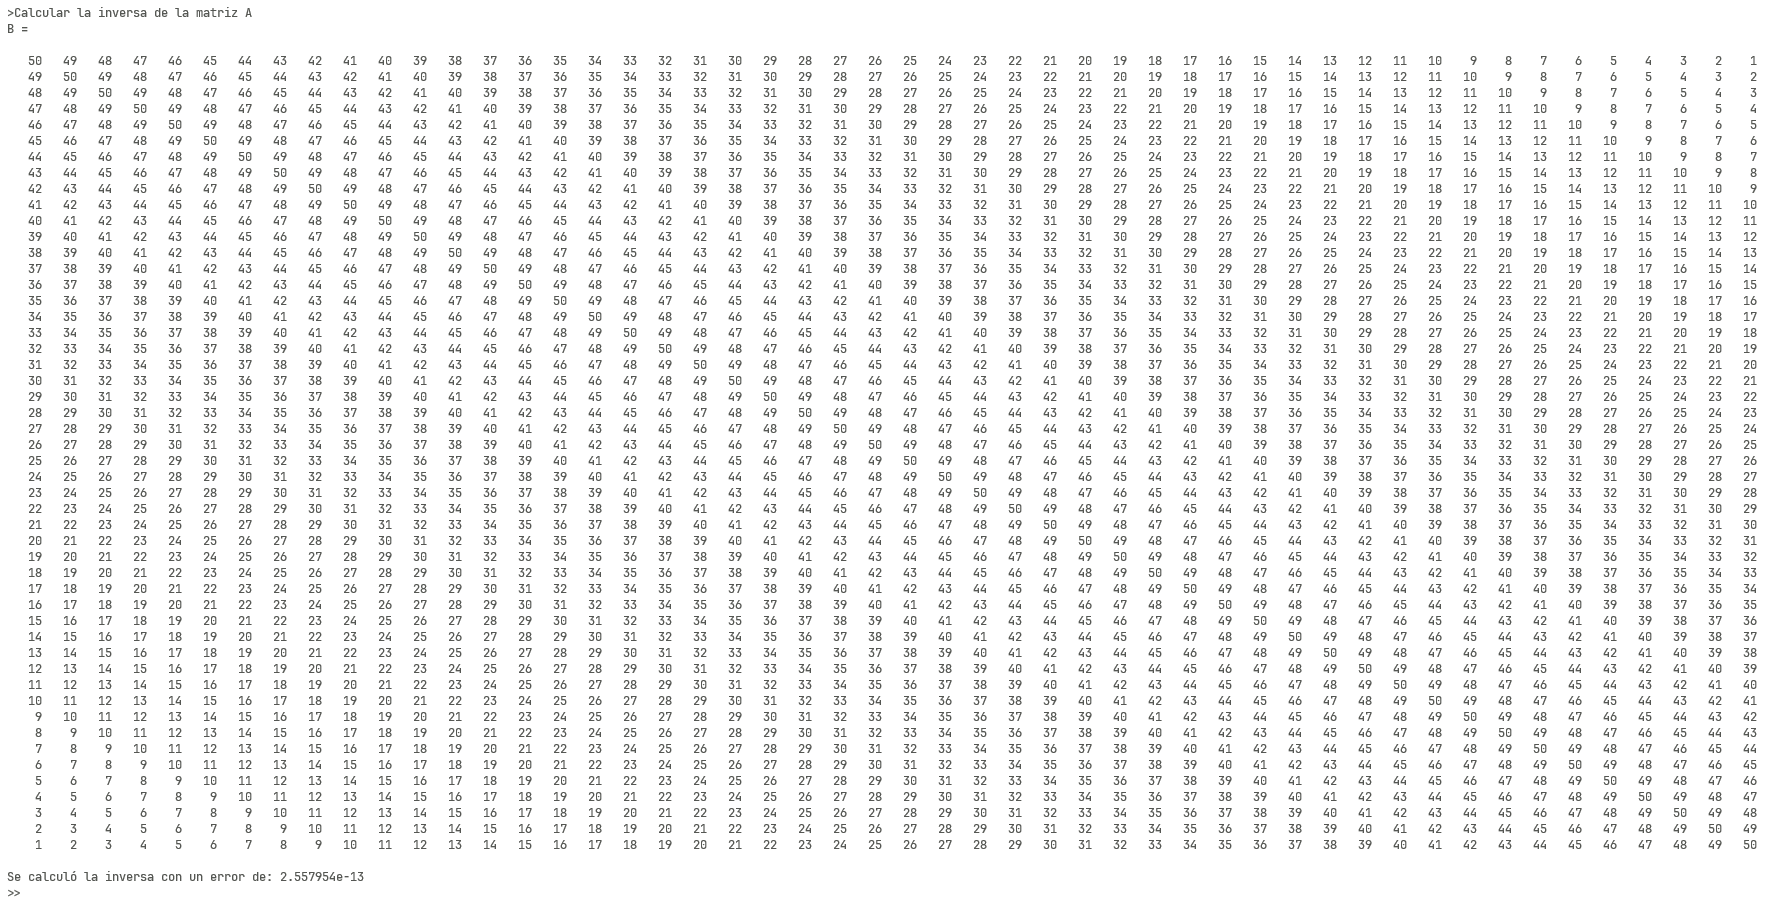
\includegraphics[width=1.1\linewidth]{ej5.resultados.png}
    \caption{Cálculo de $A^{-1}$ con $2.557954\mathrm{e}{-13}$ de error.}
    \label{fig:enter-label}
\end{figure}

\begin{figure}[H]
    \centering
    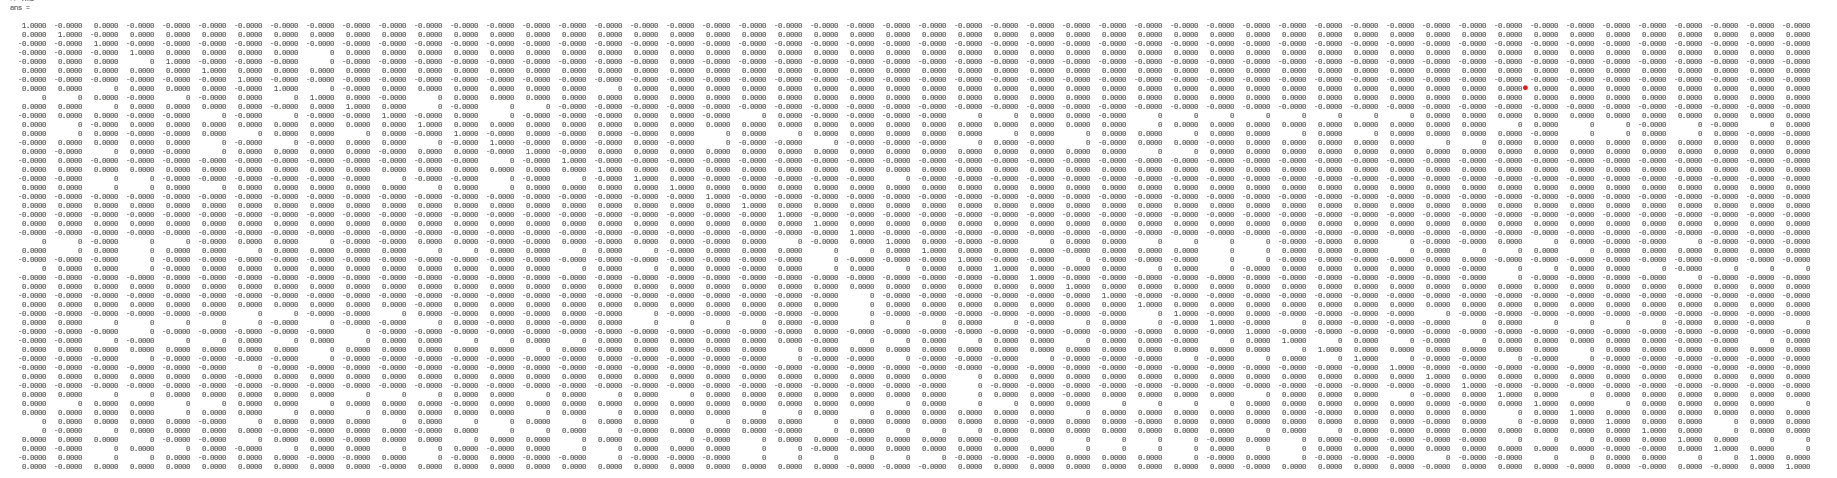
\includegraphics[width=1.15\linewidth]{ej5.resultados.2.png}
    \caption{Matric C = $A \cdot A^{-1}$ obtenida}
    \label{fig:enter-label}
\end{figure}

\begin{figure}[H]
    \centering
    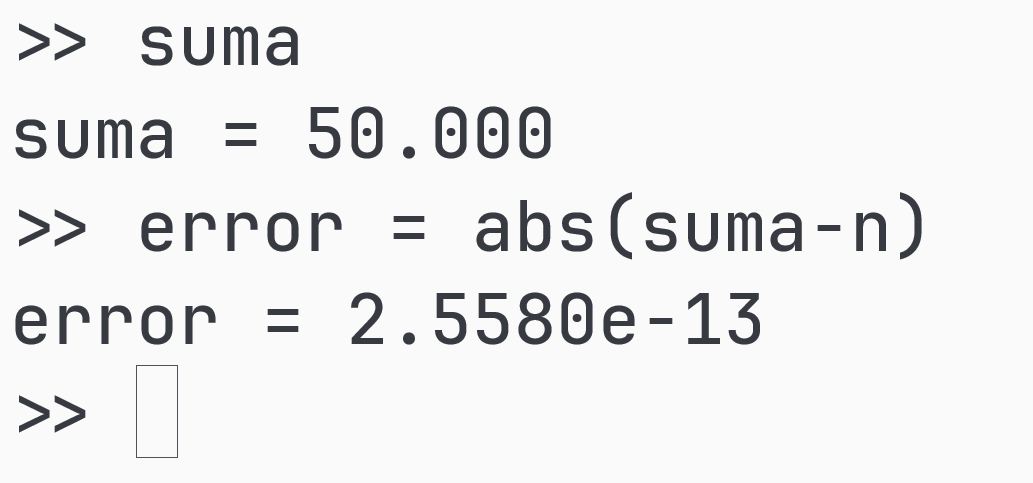
\includegraphics[width=0.8\linewidth]{ej5.resultados.3.png}
    \caption{Diferencia absoluta de la suma de los elementos de C entre n}
    \label{fig:enter-label}
\end{figure}

\begin{figure}[H]
    \centering
    \includegraphics[width=1\linewidth]{ej5.código.png}
    \caption{Código de la figura anterior}
    \label{fig:enter-label}
\end{figure}


\section{Conclusión}
Como conclusión, la teoría de errores es fundamental para el científico en computación, ya que le permite manejar los métodos numéricos con precisión y exáctictud, para resolver problemas complejos con soluciones óptimas y confiables. Esto es fundamental en problemas interdisiplinarios del mundo real, que trabajan con variables contínuas y que serán ampliamente utilizados. 

\end{document}